\documentclass[border=5mm]{standalone}
\usepackage{tikz}
\usetikzlibrary{cd}
\usetikzlibrary{decorations.pathmorphing,shapes,shapes.misc}
\begin{document}
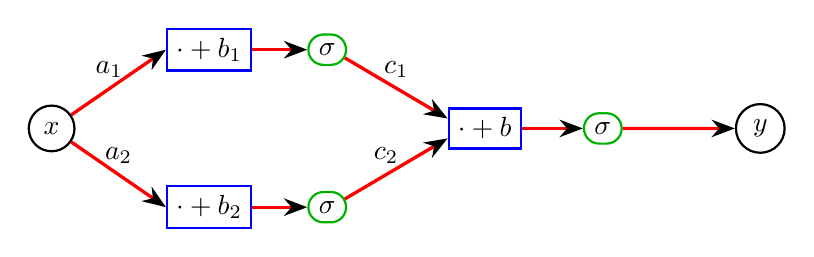
\begin{tikzpicture}
\begin{scope}[every node/.style={circle,thick,draw}]
    \node (A) at (0,0) {$x$};
    \node (D) at (9,0) {$y$};
\end{scope}
\begin{scope}[every node/.style={rectangle,thick,draw=blue}]
    \node (B1) at (2,1) {$\cdot+b_1$};
    \node (B2) at (2,-1) {$\cdot+b_2$};
    \node (B3) at (5.5,0) {$\cdot+b$};
\end{scope}
\begin{scope}[every node/.style={rounded rectangle,thick,draw=black!30!green}]
    \node (C1) at (3.5,1) {$\sigma$};
    \node (C2) at (3.5,-1) {$\sigma$};
    \node (C3) at (7,0) {$\sigma$};
\end{scope}
\begin{scope}[>={Stealth[black]},
              every edge/.style={draw=red,very thick}]
    \path [->] (A) edge node [above,pos=.4]{$a_1$}(B1.west);
    \path [->] (A) edge node [above]{$a_2$}(B2.west);
    \path [->] (B1) edge node {}(C1);
    \path [->] (B2) edge node {}(C2);
    \path [->] (C1.335) edge node [above]{$c_1$} (B3.165);
    \path [->] (C2.25) edge node [above,pos=.4]{$c_2$} (B3.195);
    \path [->] (B3) edge node {} (C3);
    \path [->] (C3) edge node {} (D);
\end{scope}
\end{tikzpicture}
\end{document}  

%
%
%
%
%
%
%
%
%
%
%
%
%
%
%
%
%
%
%
%
%
%
%
%
%
%
%
%
















